%%%%%% CMB-S4 Experimental Approach Chapter  %%%%%%%%%%%%%%%%
 
\chapter{Experimental Approach}
%\renewcommand*\thesection{\arabic{section}}

\def\nnu{N_{\mathrm eff}}
\def\gtrsim{\raise-.75ex\hbox{$\buildrel>\over\sim$}}
%%%%%%%%%%%%%%%%%%%%%%%%%%%%%%%%%%%%%%%%%%%%%%%%%%%%%%%%%%%
%%%%%%%%%%%%%%%%%%%%%%%%%%%%%%%%%%%%%%%%%%%%%%%%%%%%%%%%%%%
%%%%%%%%%%%%%%%%%%%%%%%%%%%%%%%%%%%%%%%%%%%%%%%%%%%%%%%%%%%
%%%%%%%%%%%%%%%%%%%%%%%%%%%%%%%%%%%%%%%%%%%%%%%%%%%%%%%%%%%

\section{Introduction}


The rich science case for the CMB-S4 experiment has been articulated in the first seven chapters of this Science Book.  This final chapter describes how the design of the CMB-S4 experiment flows from the science drivers.   Simulations of CMB-S4 observations, with foregrounds, the CMB, and noise, will determine the basic instrument parameters: the number and size of instrument platforms, observing bands, and the relative sensitivity in each band. Results from previous experiments will provide a foundation for detailed modeling of CMB-S4, which must incorporate systematic errors due to ground pickup, atmosphere, and beam shape, pointing, and polarization errors. The earlier experiments will also inform the choice of sample rates and scan patterns for CMB-S4 observations.

\begin{figure}[h!]
\centering
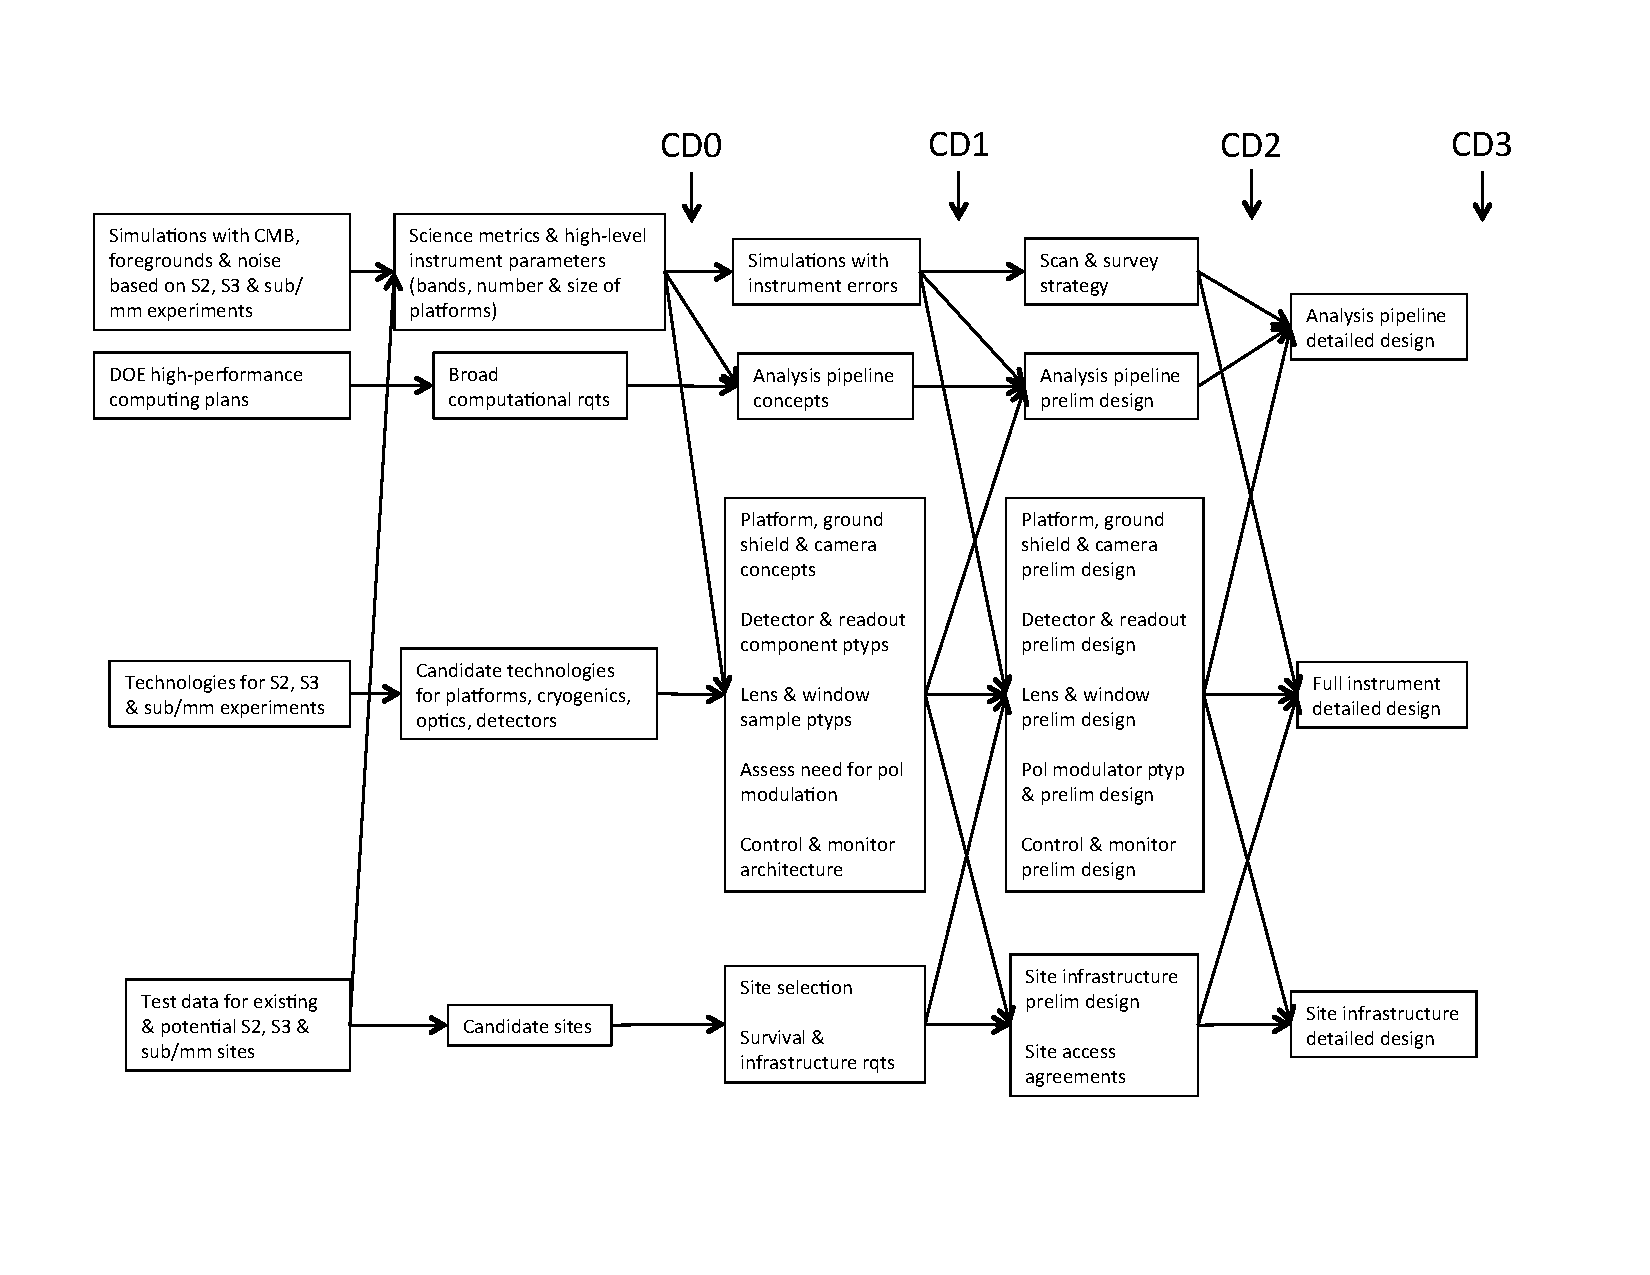
\includegraphics[trim = 0.4in 0.7in 0.8in 0.7in, clip, width=1.0\textwidth]{Instrumentation/S4TechnicalDecisionsPlan.pdf}
\caption{CMB-S4 Roadmap}
\label{fig:roadmap}
\end{figure}



A summary of the technology roadmap for CMB-S4 is shown in Fig.~\ref{fig:roadmap}.  As mentioned, the initial choice of instrument parameters is based on simulations that use maps of the CMB and astrophysical foregrounds, and measurements of instrument performance, from Stage 2 and 3 CMB experiments as well as other sub/millimeter-wavelength experiments. Technology experience from previous experiments also informs the list of candidate technologies for CMB-S4 and a rough costing for CD0. By CD1, conceptual design and critical technology development is complete, with instrument concepts feeding into the analysis pipeline design and site infrastructure design. The coupling between instrument, analysis pipeline, and site infrastructure design continues through preliminary design, which defines the baseline project at CD2, and detailed design, which delivers a construction-ready project at CD3.

\section{Technical Development}

\subsection{Detector Arrays}

\begin{figure}[t]
\centering 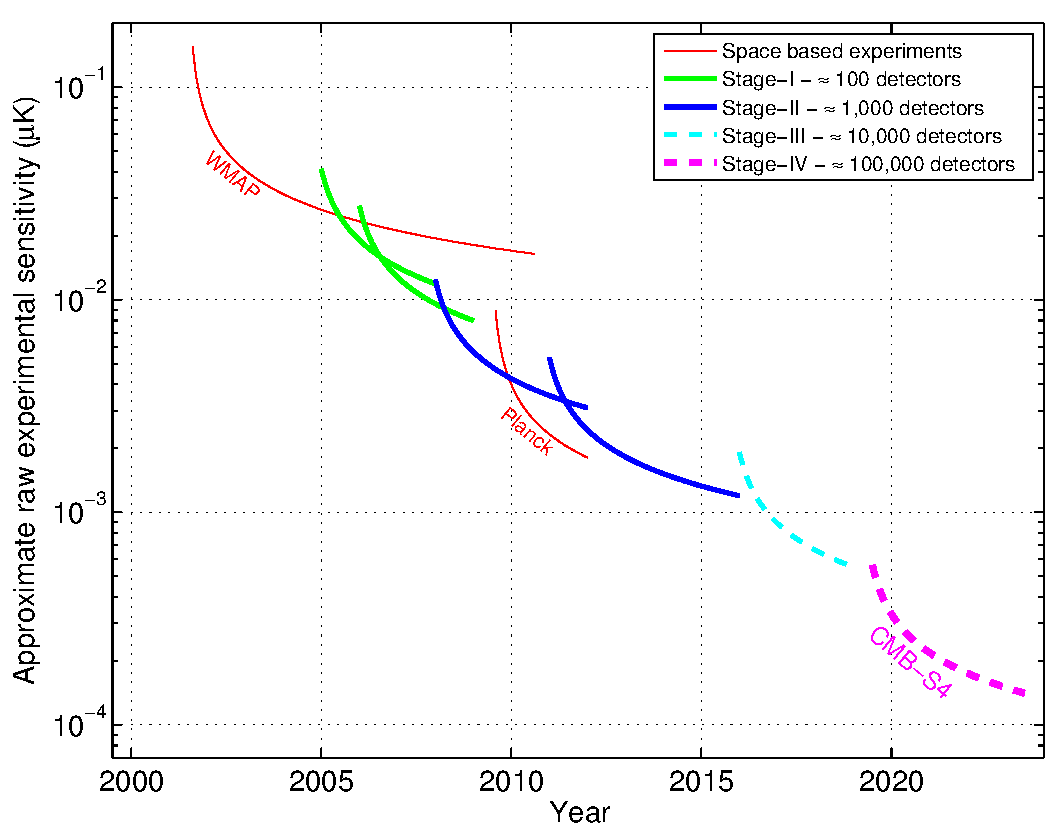
\includegraphics[width=0.75\textwidth]{Intro/expt_progress.pdf}
\caption{Plot illustrating the evolution of the raw sensitivity of CMB
  experiments, which scales as the total number of
  bolometers. Ground-based CMB experiments are classified into Stages
  with Stage II experiments having $O$(1000) detectors, Stage III
  experiments having $O$(10,000) detectors, and a Stage IV experiment
  (such as \cmbexp) having $O$(100,000) detectors.}
\label{fig:expt_progress}
\end{figure}

State-of-the-art CMB detectors are sensitivity-limited where the dominant
noise in an individual detector element comes from shot noise arising
from the arrival time of the photons. Thus, achieving the required
\cmbexp\ sensitivity requires increasing the number of detected modes,
which is straightforward to achieve by increasing the number of
detectors (see Fig.~\ref{fig:expt_progress}). \cmbexp\ will have 500
times more detectors than the current state-of-the-art Stage 2
experiments, 30 times more than planned Stage 3 experiments, making
scaling the primary technical challenge of \cmbexp.

\begin{figure}[t]
\centering
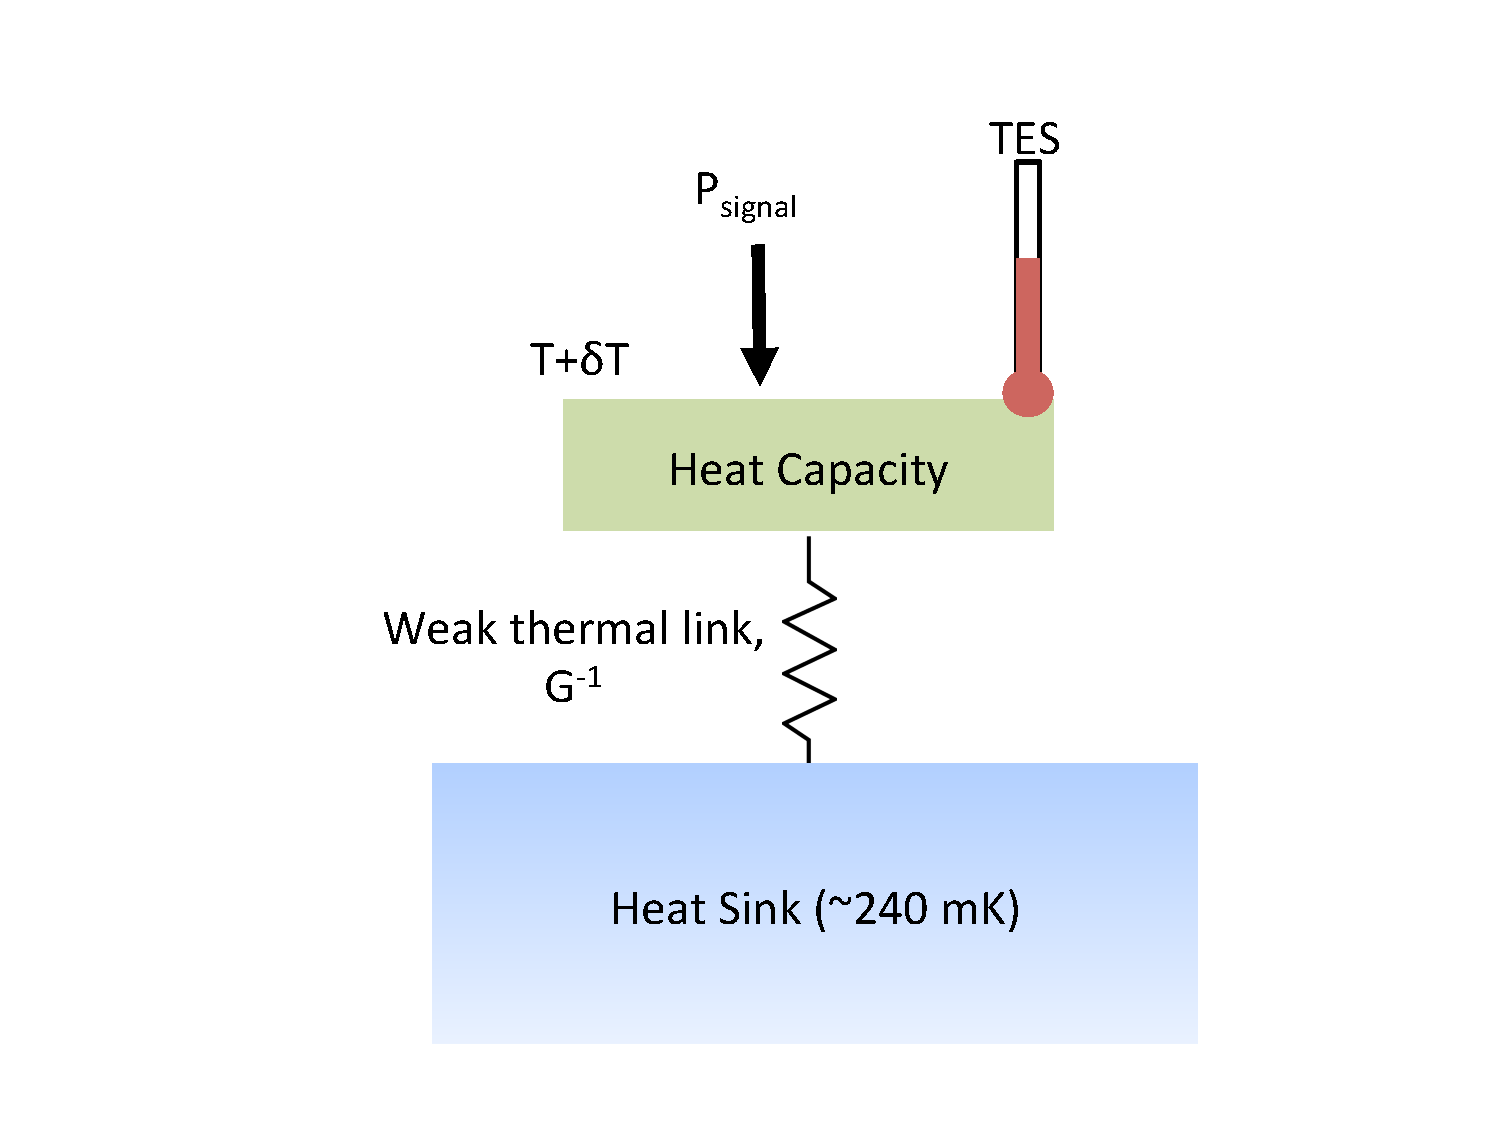
\includegraphics[trim=0.7in 0 1.5in 0,clip,scale=0.3]{Instrumentation/ThermalCircuit.pdf}
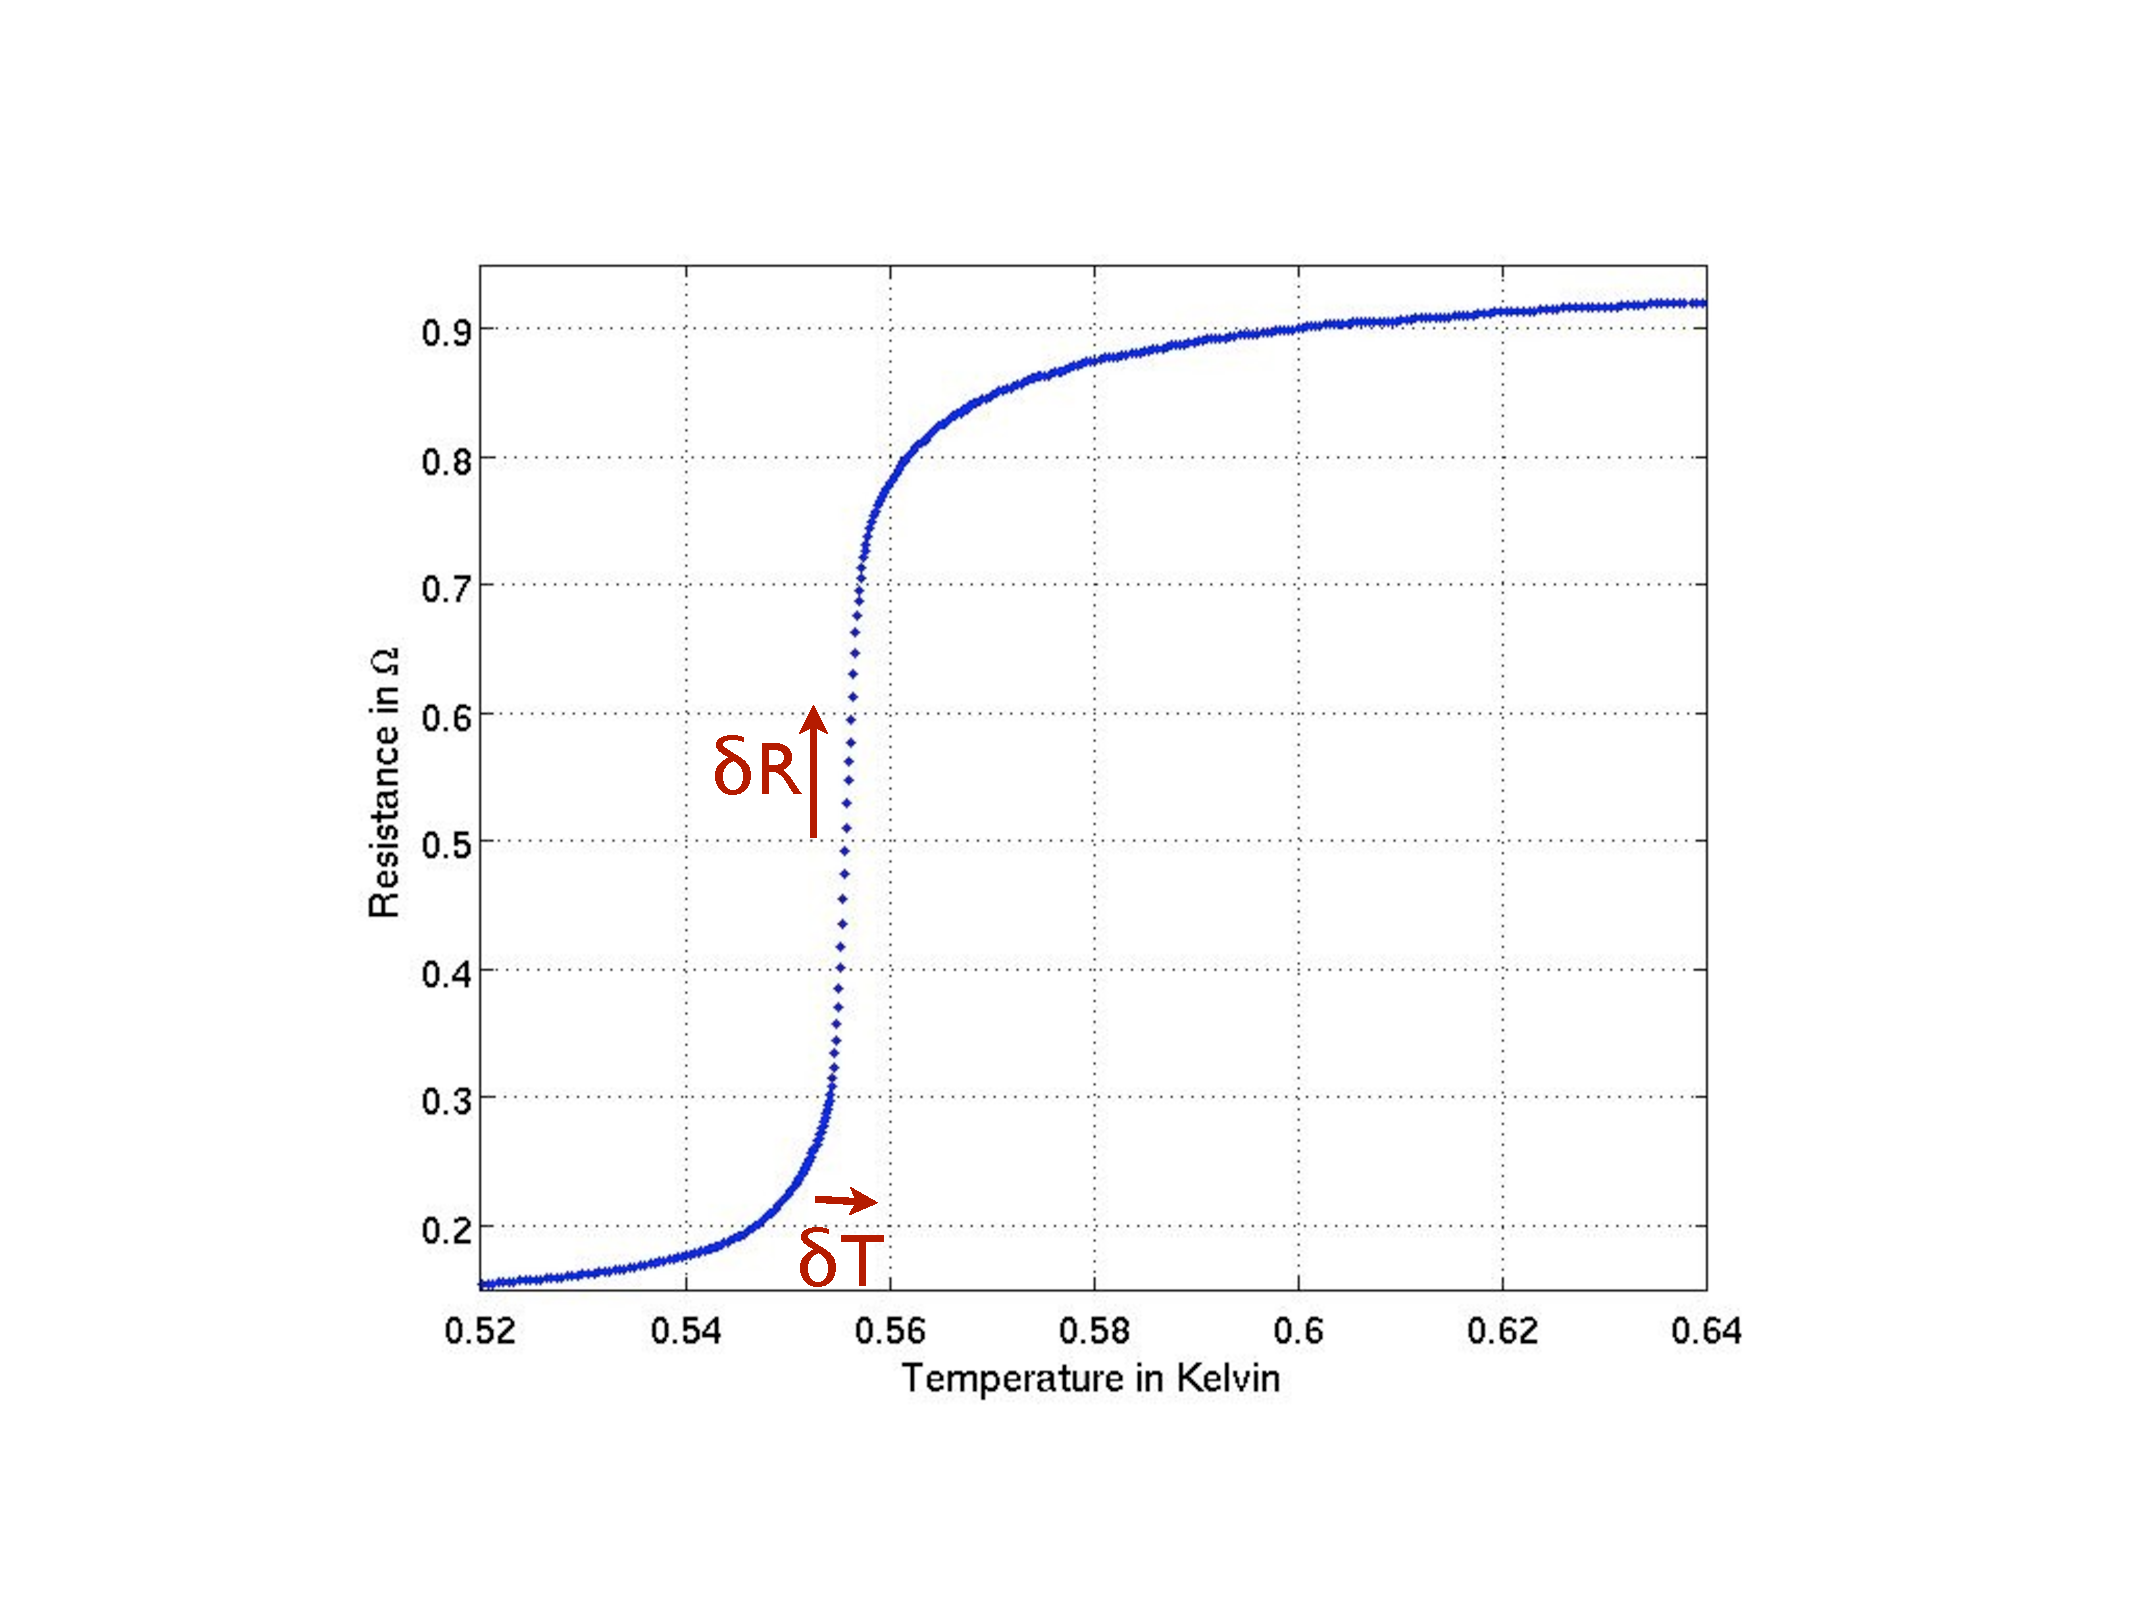
\includegraphics[trim=0.4in 0.4in 0.1 0,clip,scale=0.23]{Instrumentation/RvsT.pdf}
\vskip 0pt
\caption{Left: Illustration of a thermal circuit for a typical
  Transition Edge Sensor (TES) detector highlighting the principles of
  signal detection. A weakly thermally sunk heat capacity absorbs
  power, P$_{\rm signal}$, which is to be measured. Variations in the
  absorbed power change the heat capacity's temperature, which is
  measured by a TES operating under strong electro-thermal
  feedback. Right: Plot of resistance versus temperature for a typical
  TES illustrating the principles of negative electro-thermal
  feedback~\cite{irwin:1998}. The TES is voltage biased into the
  middle of its superconducting-to-normal transition. Small changes in
  the TES temperature produce large changes in the TES
  resistance. Since the TES is voltage biased, an increase (or
  decrease) in the temperature produces an increase (or decrease) in
  the resistance leading to a decrease (or increase) in the Joule
  heating power supplied by the bias. This canceling effect
  corresponds to a strong negative electro-thermal feedback making the
  current through the TES nearly proportional to P$_{\rm signal}$.}
\label{fig:TEScartoon}
\vskip -12pt
\end{figure}


Towards this end, the baseline plan is that \cmbexp\ will utilize Transition Edge Sensor (TES)
bolometers as its detector technology, although alternate technologies being developed
by the community such as MKIDs will be evaluated.  
%\footnote{We note that
%  at the lowest frequencies envisioned, $\sim40$ GHz, MMIC-amplifier
%  or new superconducting amplifier technologies may be practical.} 
A TES is an ultra-sensitive thermometer consisting of a thin
superconducting film weakly heat-sunk to a bath temperature much lower
than the superconductor $T_{c}$ (see Fig.~\ref{fig:TEScartoon},
left). The principles of operation are simple to understand. By
supplying electrical power to the TES, we can raise the temperature of
the sensor so that the film is in the middle of its
superconducting-to-normal transition (see Fig.~\ref{fig:TEScartoon},
right). If the electrical power is supplied via a voltage bias, a
negative feedback loop is established~\cite{irwin:1998}. Small changes
to the TES temperature, arising from thermal fluctuations (noise) or
changes in the absorbed power from a source (signal), lead to large
changes in the TES resistance. The change in resistance creates a
canceling effect because increases (or decreases) in temperature
produce decreases (or increases) in Joule heating power. This negative
electro-thermal feedback is very strong because the transition is very
sharp. It linearizes the detector response and expands the detector
bandwidth.

The TES has a number of strengths making it an attractive technology to
pursue for \cmbexp. First, TES detectors are fabricated via
micro-machining of thin films deposited on silicon wafer
substrates. As a consequence, the fundamental production unit for TES
devices are arrays of detectors (see Fig.~\ref{fig:tes_array}), an
important attribute when considering the production of the 500,000
detectors required by \cmbexp.  Second TES devices are low-impedance
($\le$1~$\Omega$) and can be multiplexed with modern-day
Superconducting QUantum Interference Device (SQUID)
multiplexers~\cite{fmux,tmux,umux}. Multiplexed readouts are important
for operating large detector arrays at sub-Kelvin temperatures and are
essential for \cmbexp. Lastly, TES detectors have been successfully
deployed as focal planes at the forefront of CMB measurements.



The TES was invented by HEP for detecting Dark Matter and
neutrinos. Its subsequent integration into CMB focal planes has
enabled kilo-pixel arrays realizing the Stage 2 CMB program and
ushering in an era of unprecedented sensitivity. TES-based CMB
detectors are the favored technology among Stage 2 and proposed Stage
3 experiments, and have a clear path to the sensitivities required
by \cmbexp. The ubiquity of TES detectors for CMB illustrates the
direct connection between HEP-invented technology and CMB science.


\begin{figure}[t!]
\centering
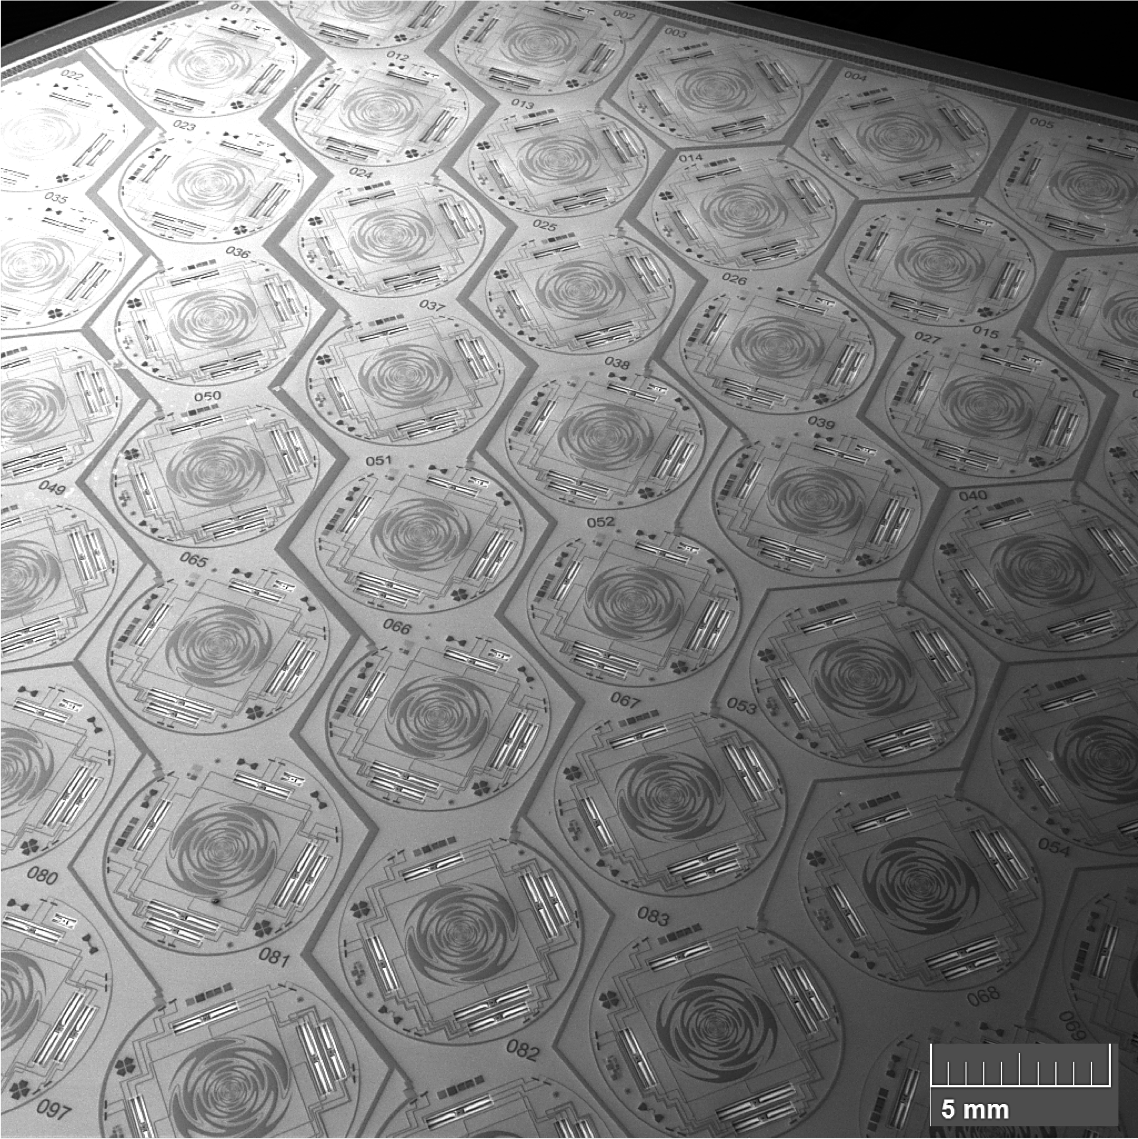
\includegraphics[width=0.4\textwidth]{Instrumentation/ANL-Fab-Detector-Array.png}
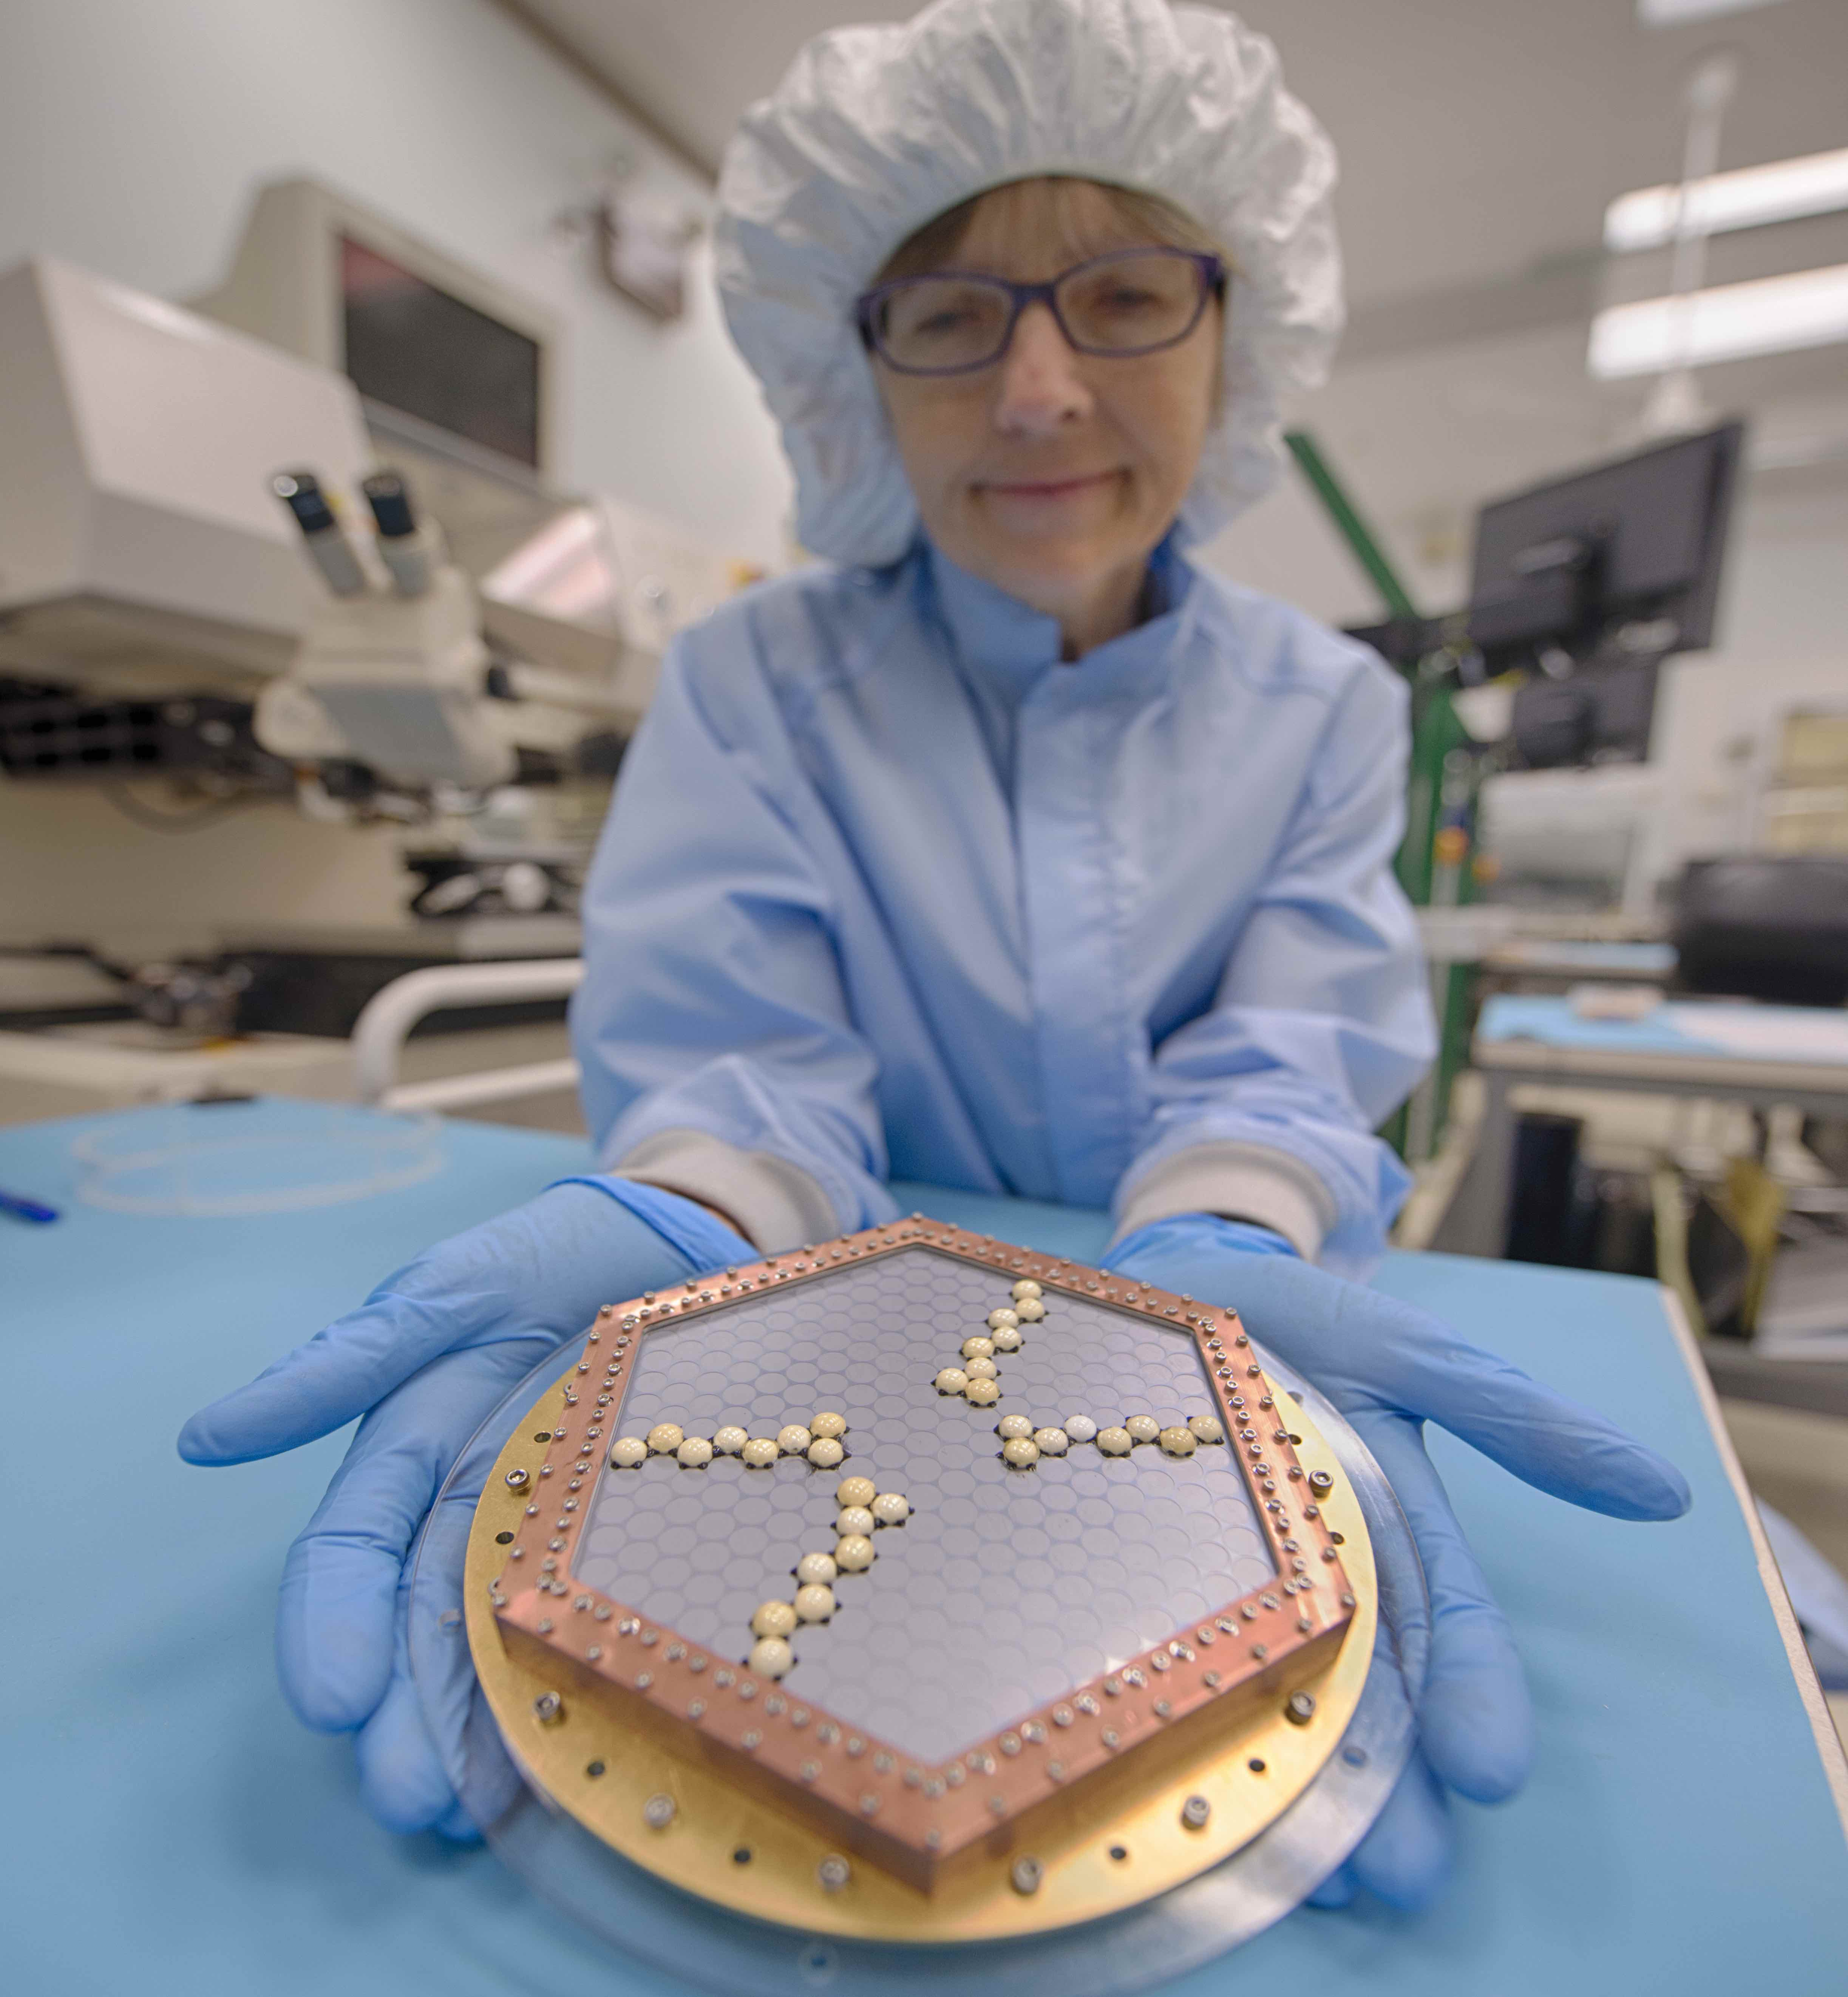
\includegraphics[trim=0.0in 0.8in 0.0in 4.5in,clip=true,width=0.4\textwidth]{Instrumentation/FNAL_spt3g_wafer_assembly.jpg}
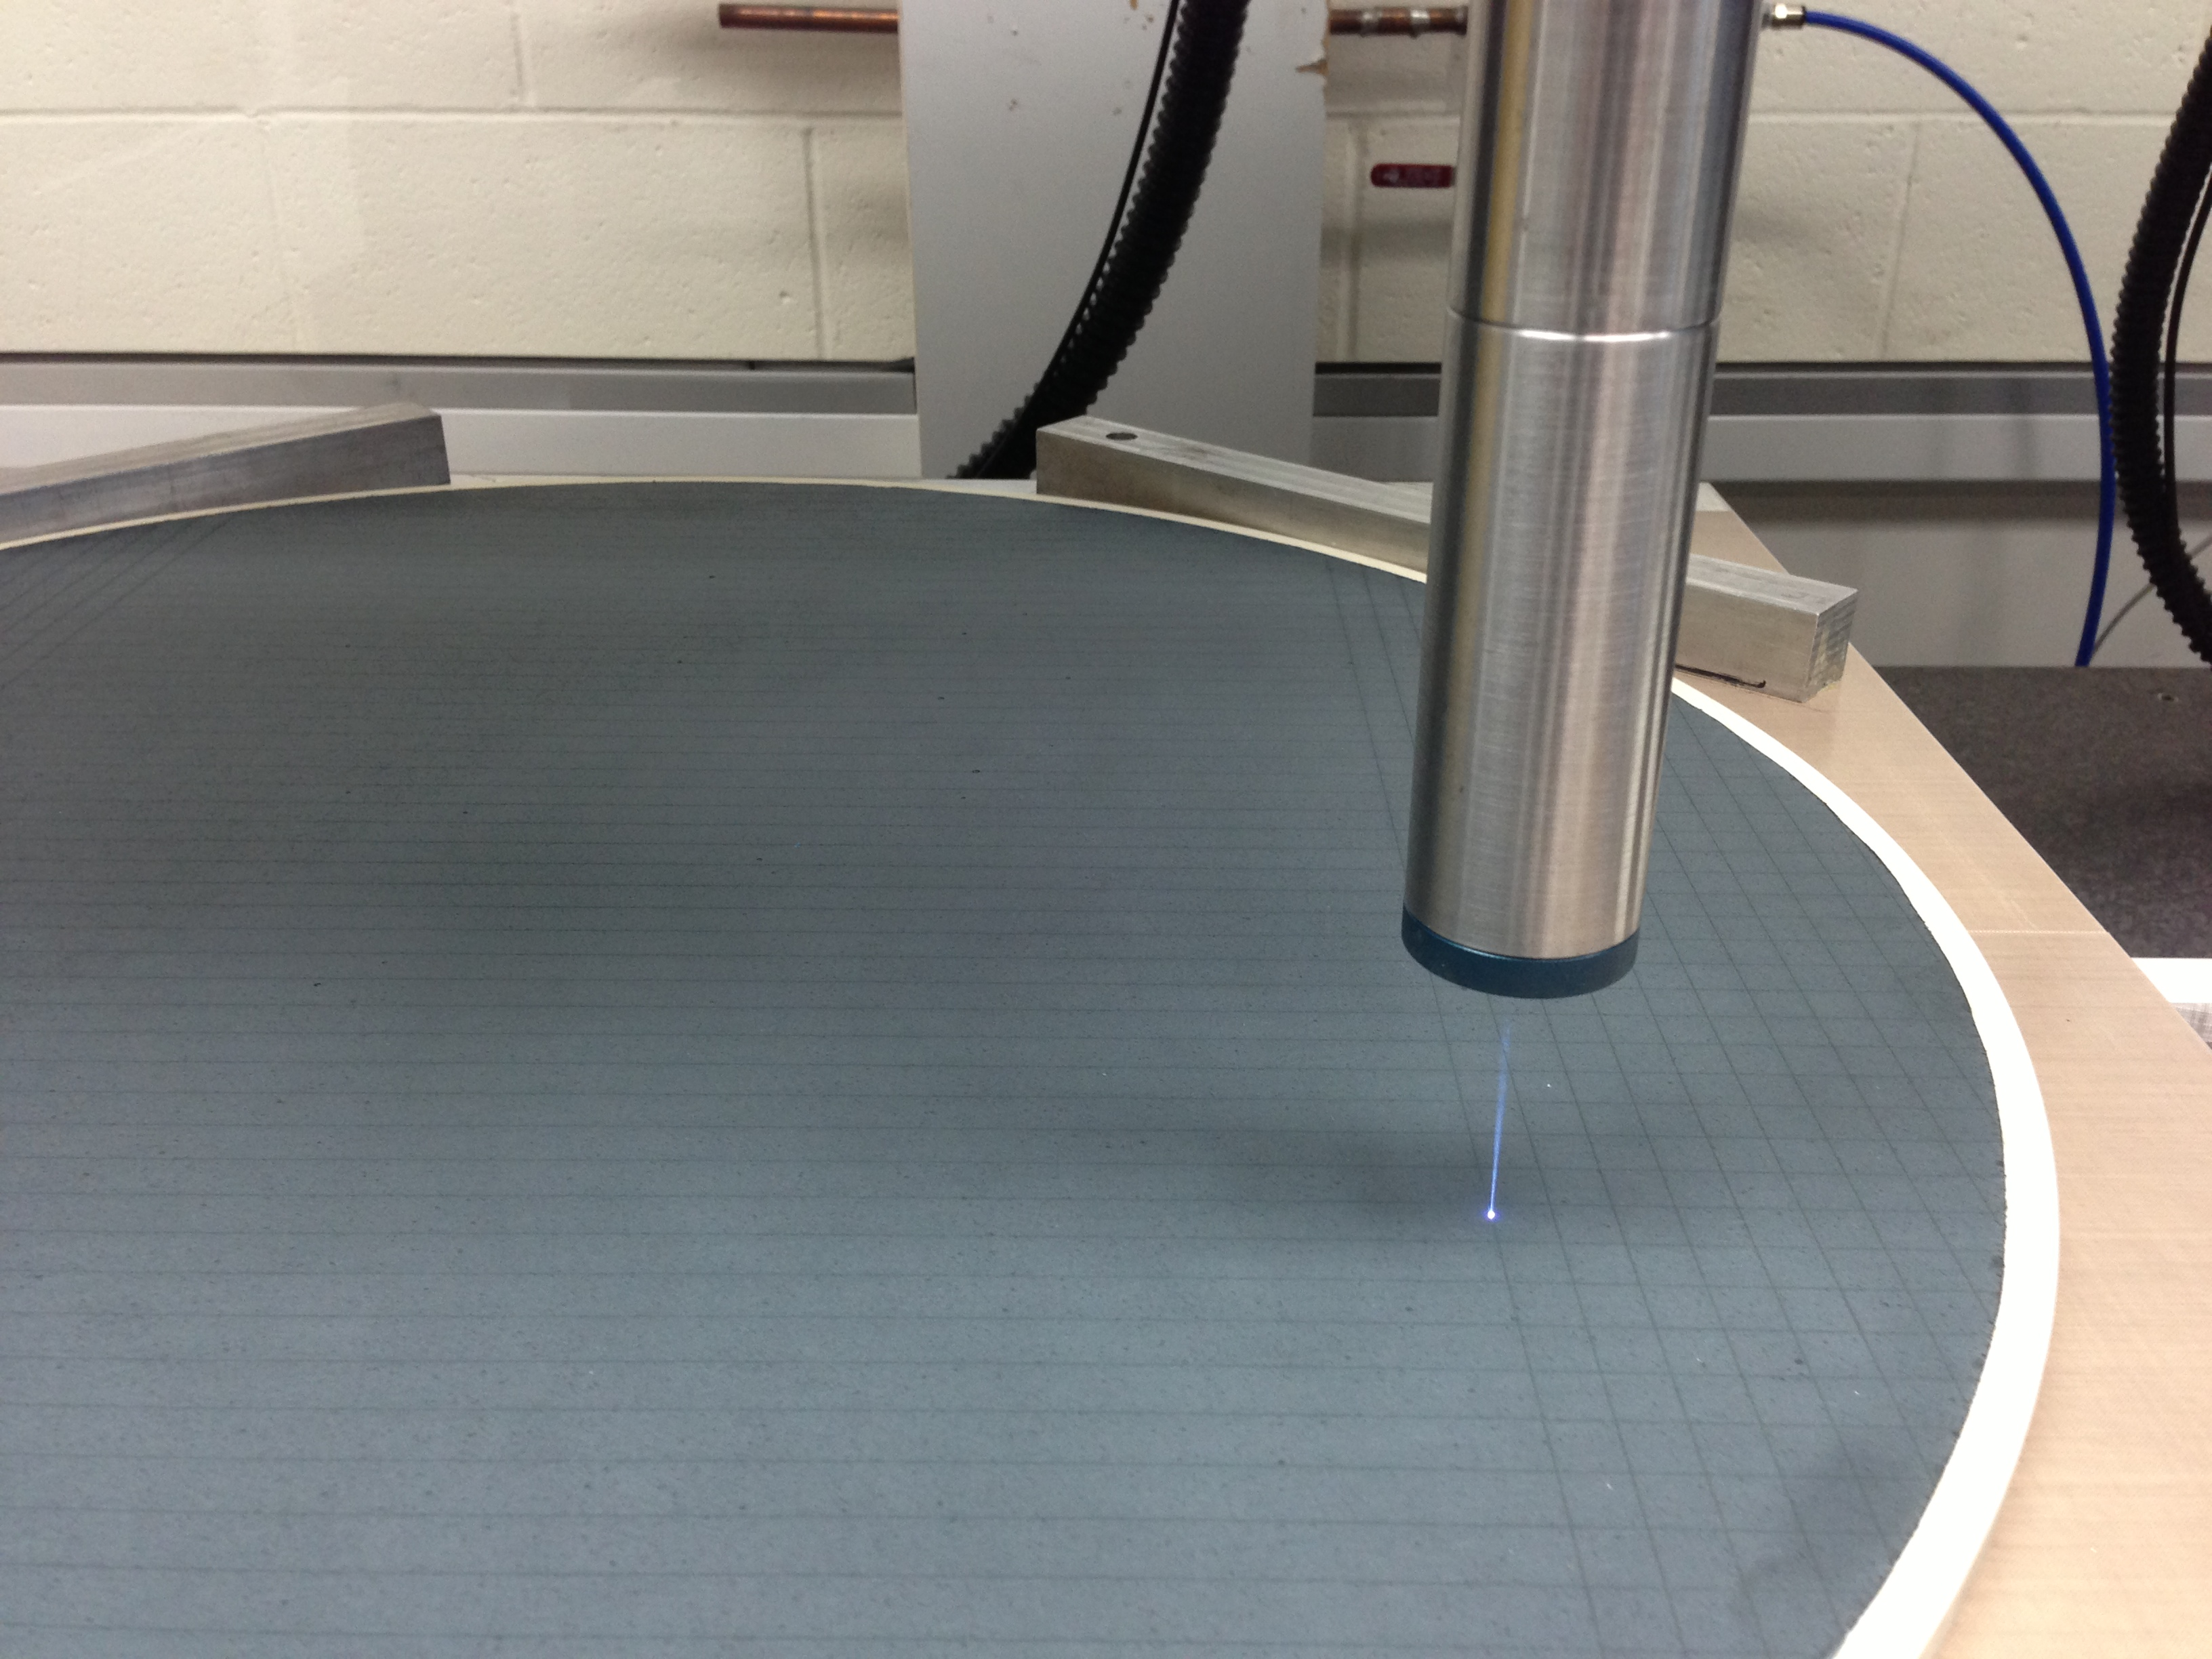
\includegraphics[width=0.4\textwidth]{Instrumentation/SLAC_laser.jpg}
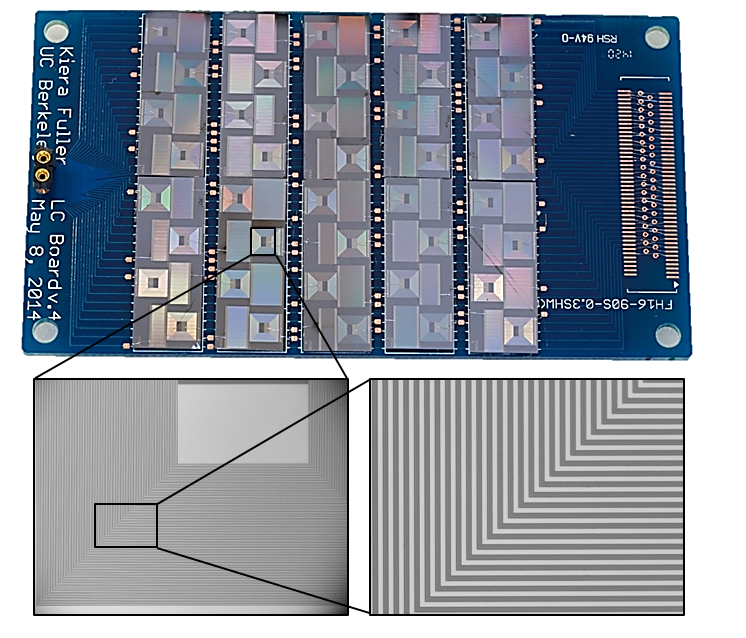
\includegraphics[width=0.4\textwidth]{Instrumentation/LCChipInset2.png}
\caption{Illustrations of technology development at each of the four DOE labs working on CMB-S4.  Clockwise from upper left:  Multichroic bolometer array fabricated at ANL; Array module assembled at Fermilab; Superconductor resonators for bolometer readout fabricated at LBNL; and Laser-dicing of an optical filter at SLAC.}
\label{fig:tes_array}
\end{figure}



\subsubsection{Development of mass production capability at the national labs}

Delivering a half-million background-limited bolometers necessitates a
change in the execution of the U.S.\ ground-based CMB program. The
current program consists of a number of independent (primarily
university) efforts, each focused on the development and delivery of
their own instrument. The involvement of HEP in the current process
has been through small investments targeted at specific technical
contributions. 
Current detector fabrication R\&D for each of these independent efforts aims to field $\sim$15,000 detectors over the course of three years with throughput limited by fabrication and testing resources. This level of production capacity is sufficient for Stage 3 experiments, but is inadequate for the challenges of \cmbexp. 
Realizing \cmbexp\ will require a radical change in
this approach where HEP resources take the leading role. Of particular
importance is an increased participation and support of national labs
to provide resources which are unavailable to university groups. In
particular, 1) leveraging micro-fabrication tools and expertise
available at multi-purpose national labs is essential for the
successful fabrication of the \cmbexp\ detectors, 2) supporting
the computing infrastructure to support the greatly increased data
rate, dataset size and analysis complexity, 
and 3) leveraging experience and resources for partnering with industry and the commercial sector.

The \cmbexp\ experimental program will build on the success of Stage
2 and 3 CMB experiments.  It will be a coherent effort
incorporating resources from both national labs and university groups.

The necessary steps required for developing array fabrication ability
for CMB-S4 include:

\begin{itemize}

\item {\bf Improved Production Reliability} The favored technology for
  \cmbexp\ are TES bolometers coupled through superconducting
  microstrip. Critical for the TES technology is reliable and optimal
  superconducting microstrip performance at millimeter
  wavelengths. Recent work on microstrip-coupled CMB detectors have
  demonstrated that it is possible to make superconducting microstrip
  which is virtually loss-less at the required
  frequencies~\cite{sptpol150}; however, the fabrication yield needs
  to be improved for \cmbexp. Thus, one of the principle components of
  the \cmbexp\ program is developing a reliable mass production
  process. Such work requires well maintained tooling, dedicated
  materials deposition, and understanding and control of all the
  materials dependent loss mechanisms.


\item {\bf Increased Production Volume and Throughput} Achieving
  $O$(500,000) TES detectors demands new investment into TES array
  production resources. The required production throughput needs
  access to micro-fabrication resources with exclusive control of the
  thin film deposition systems. This exclusive access to
  microfabrication tooling falls squarely within the domain of
  national labs, or by technology transfer to a qualified industrial partner. Additionally, an extensive program of detector
  testing, characterization, and quality control is crucial for the
  mass production of 500,000 TES bolometers. This requirement will be
  met by establishing test facilities and organizing a quality
  assurance program among the universities and national labs.

\end{itemize}



\subsection{Multiplexed Detector Readout}

 Multiplexed TES readouts are
  required for implementing focal planes with more than 1000 detector
  elements and will continue to be an active component of the
  \cmbexp\ R\&D program. Modest improvements over existing fielded
  Stage 2 multiplexer technology will be sufficient for the needs of
  \cmbexp. However, recent developments with microwave-based readout
  techniques for TES detectors may lead to new multiplexer technologies
  with broader applicability and lower cost, and could be synergistic
  with microwave kinetic inductance detector (mKID) readout development efforts.   


\subsection{Telescope Architecture and Reimaging Optics }

There are several types of telescope architectures that are currently
being used successfully in Stage 2 experiments.   Most telescopes
are reflector type (mirror-based), although the BICEP/KECK series of experiments are
refractors (lens-based).   Both types of telescope offer high performance, but 
the refractors are limited in diameter and therefore angular resolution.  
In reflector telescopes, both standard Gregorian and crossed Dragone 
designs have successfully been used.   

As part of the CMB-S4 technology roadmap, optics studies will be performed
to develop a design with both large optical throughput to accommodate large
detector arrays and high polarization purity.

The large size of the
  \cmbexp\ focal planes together with the required sub-Kelvin
  operating temperature necessitates the development of new broad-band
  large aperture  refractive reimaging optics which permit high throughput at
  millimeter wavelengths while blocking infrared thermal
  emission. Upcoming Stage 3 experiments will serves as a proving
  ground for some new cryogenic optics technologies. \cmbexp\ will
  build on these Stage 3 accomplishments with the goal of developing
  manufacturing techniques to yield a large number of customized
  cryogenic optics with optimal performance.

\subsection{Polarization Modulation}

Polarization modulators, such as continuously rotated half-wave plates that are used in 
ABS, POLARBEAR, and AdvACT, and a variable-delay polarization modulator (VPM) used
in CLASS can give improved rejection of atmospheric fluctuation noise and a reduction 
in intensity-to-polarization conversion when compared to bolometer differencing.    In the
CMB-S4 technology roadmap, we will use the experience from Stage 3 experiments to assess
the tradeoffs of using polarization modulators and we will develop large-throughput and 
high-bandwidth modulators.  




     
     
%\bibliography{cmbs4}

%%
%% Populate the .bib file with entries from SPIRES Bibtex (preferred)
%% or ADS Bibtex (if no SPIRES entry).
%%  SPIRES will also supply the CITATION line information; please include it.
%%


